%\documentclass[english,10pt]{beamer}
\documentclass[english,handout]{beamer}






 
%\usepackage{mathptmx}
%\renewcommand{\sfdefault}{lmss}
\usepackage[T1]{fontenc}
%\usepackage[latin9]{inputenc}
\usepackage[utf8]{inputenc}

\synctex=-1

\usefonttheme{professionalfonts}

%\setbeamertemplate{navigation symbols}{}
%\setbeamertemplate{caption}[numbered]


\useinnertheme{rectangles}
%http://tex.stackexchange.com/questions/11168/change-bullet-style-formatting-in-beamer

 \AtBeginDocument{
  \addtolength\abovedisplayskip{-0.4\baselineskip}%
  \addtolength\belowdisplayskip{-0.4\baselineskip}%
}%change the space between text lines and the math formula


\usepackage{pifont}
%Postscript ZipfDingbats font
%the command \ding{number}, will print the specified symbol

\usepackage{fontawesome}
%icon package
\DeclareFontFamily{U}{FontAwesomeOne}{}
\DeclareFontShape{U}{FontAwesomeOne}{m}{n}{<-> FontAwesome--fontawesomeone}{}
\DeclareRobustCommand\FAone{\fontencoding{U}\fontfamily{FontAwesomeOne}\fontseries{m}\fontshape{n}\selectfont}
\DeclareFontFamily{U}{FontAwesomeTwo}{}
\DeclareFontShape{U}{FontAwesomeTwo}{m}{n}{<-> FontAwesome--fontawesometwo}{}
\DeclareRobustCommand\FAtwo{\fontencoding{U}\fontfamily{FontAwesomeTwo}\fontseries{m}\fontshape{n}\selectfont}
\DeclareFontFamily{U}{FontAwesomeThree}{}
\DeclareFontShape{U}{FontAwesomeThree}{m}{n}{<-> FontAwesome--fontawesomethree}{}
\DeclareRobustCommand\FAthree{\fontencoding{U}\fontfamily{FontAwesomeThree}\fontseries{m}\fontshape{n}\selectfont}

%ftp://ftp.dante.de/tex-archive/fonts/fontawesome/doc/fontawesome.pdf
%http://tug.ctan.org/info/symbols/comprehensive/symbols-a4.pdf


\usepackage{amsmath,amssymb,amsfonts,bm,mathrsfs,mathtools}

\usepackage{tikzsymbols}
%\usepackage[tikz]{bclogo}



\usepackage{perpage}
\MakePerPage{footnote} %reset for each page
%\renewcommand{\thefootnote}{\fnsymbol{footnote}} %use symbol, limit less than 9 symbols



%%%% HIGHTLIGHT  and annotation &=%%%%%%%%
\usepackage{color,xcolor}
 \usepackage{todonotes}

\usepackage[normalem]{ulem}

\usepackage[many]{tcolorbox}

\tcbset{fonttitle=\scriptsize}
\tcbset{highlight math style={enhanced,
  colframe=red!40!black,colback=yellow!20!white,arc=2pt,boxrule=.2pt,
  }}
  \newtcbox{\otherbox}[1][]{nobeforeafter,math upper,tcbox raise base,
enhanced,frame hidden,boxrule=0pt,interior style={top color=green!10!white,
bottom color=green!10!white,middle color=green!50!yellow},
fuzzy halo=1pt with green,#1}
%%\tcbhighmath{math here}
%% \otherbox{math here}



%%%%% HIGHLIGHT %%%%%%
\newcommand{\hb}[1]{{\color{blue}{#1}}}
%\noindent\rule{\textwidth}{.5pt}

%:
\usepackage{soul}

\newcommand\hcancel[2][black]{\setbox0=\hbox{$#2$}%
\rlap{\raisebox{.45\ht0}{\textcolor{#1}{\rule{\wd0}{1pt}}}}#2}
%cross to delete

\newcommand{\mcb}[2]{\colorbox{#1}{$\displaystyle #2$}}
%highlight math

\newcommand{\hlfancy}[2]{\sethlcolor{#1}\hl{#2}}
%specified color , for\hl

\newcommand\myhl{\bgroup\markoverwith
  {\textcolor{yellow}{\rule[-.5ex]{2pt}{2.5ex}}}\ULon}



\mode<presentation>{ \usetheme{boxes} }

%write Matlab code
\usepackage{listings}
 \definecolor{dkgreen}{rgb}{0,0.6,0}
\definecolor{gray}{rgb}{0.5,0.5,0.5}
\definecolor{mauve}{rgb}{0.58,0,0.82}
\lstset{frame=tb,
  language=Matlab,
  aboveskip=3mm,
  belowskip=3mm,
  showstringspaces=false,
  columns=flexible,
  basicstyle={\small\ttfamily},
  numbers=none,
  numberstyle=\tiny\color{gray},
  keywordstyle=\color{blue},
  commentstyle=\color{dkgreen},
  stringstyle=\color{mauve},
  breaklines=true,
  breakatwhitespace=true
  tabsize=3
}

\usepackage[lastexercise]{exercise}

\newtheorem{ex}{Exercise}
\newtheorem{property}{Property}
\newtheorem{ag}{Algorithm}
\newtheorem{remark}{Remark}
\newtheorem{den}{definition}
\newtheorem{assumption}{Assumption}


\usepackage[nosolutionfiles]{answers}
\Newassociation{sol}{Solution}{ans}



\usepackage{empheq}
\usepackage{comment}
%\usepackage{lscape}
\usepackage{multirow}
\usepackage{url,hyperref}

\hypersetup{
 %   bookmarks=true,         % show bookmarks bar?
    unicode=false,          % non-Latin characters in Acrobat's bookmarks
    pdftoolbar=true,        % show Acrobat's toolbar?
    pdfmenubar=true,        % show Acrobat's menu?
    pdffitwindow=false,     % window fit to page when opened
    pdfstartview={FitH},    % fits the width of the page to the window
    pdftitle={My title},    % title
    pdfauthor={Author},     % author
    pdfsubject={Subject},   % subject of the document
    pdfcreator={Creator},   % creator of the document
    pdfproducer={Producer}, % producer of the document
    pdfkeywords={keyword1} {key2} {key3}, % list of keywords
    pdfnewwindow=true,      % links in new window
    colorlinks=true,       % false: boxed links; true: colored links
    linkcolor=red,          % color of internal links (change box color with linkbordercolor)
    citecolor=green,        % color of links to bibliography
    filecolor=magenta,      % color of file links
    urlcolor=cyan           % color of external links
}


\usepackage{subfigure,epsfig,graphicx,graphics}

\DeclareGraphicsRule{.tif}{png}{.png}{`convert #1 `dirname #1`/`basename #1 .tif`.png}
   \DeclareGraphicsExtensions{.pdf}




\newcommand{\hw}{ {\underline{\tt Homework }} }
\newcommand{\hws}{ {\underline{\tt Homework$\star$}} }
\newcommand{\optional}{ {\it optional} }

\newcommand{\MATLAB}{ \texttt{MATLAB}}
\newcommand{\python}{ \texttt{python}}
\newcommand{\Rlang}{ \texttt{R}}
\newcommand{\SAS}{ \texttt{SAS}}
\newcommand{\MC}{Markov Chain}


\newcommand{\tm}{transition matrix}
\newcommand{\rv}{random variable}
\newcommand{\spl} {supervised learning }
 

\newcommand{\dis}{\underline{\tt discussion}: }
\newcommand{\pri}{\underline{\tt principle}: }




\newcommand{\bq}{\scalebox{6}{\textbf{?} }}
\newcommand{\sq}{\scalebox{2}{\textbf{?} }}
\newcommand{\ck} {  {\scalebox{0.8} {\Interval}   } }

\newcommand{\eps}{\varepsilon}
\newcommand{\To}{\longrightarrow}

% 
\newcommand{\Dcal}{\mathtt{D}}
\newcommand{\Hcal}{\mathcal{H}}
\newcommand{\Ecal}{\mathcal{E}}
\newcommand{\Xcal}{\mathcal{X}}
\newcommand{\Ycal}{\mathcal{Y}}
\newcommand{\Zcal}{\mathcal{Z}}

%%Calculus 

\renewcommand{\d}{\ensuremath{\mathrm{d}}}
\newcommand{\dt}{ \ensuremath{\mathrm{d} t } }
\newcommand{\dx}{ \ensuremath{\mathrm{d} x} }
\newcommand{\dy}{ \ensuremath{\mathrm{d} y } }

%indicator function
\newcommand{\indf}{ \ensuremath{\mathbf{1} } }



%probability
\newcommand{\p}{ \mathbb{P}}
\newcommand{\prob}{{\Pr}}
\newcommand{\PP}{\mbox{PP}}%Poisson process
%condition prob
\newcommand{\cPr}[2]{{\Pr\left(#1\mid #2\right)}}

\newcommand{\FF}{{\mathbb{F}}}

\newcommand{\e}{ \operatorname{\mathbb E}}
\newcommand{\Var}{\operatorname{\mathbb{V} }}
\newcommand{\var}{\operatorname{\text{Var} }}
\newcommand{\MSE}{\operatorname{\text{MSE} }}

\newcommand{\Std}{\operatorname{std}}
\newcommand{\Cov}{\operatorname{cov}}

%Matrix  %mathbf
\newcommand{\Pb}{{\mathbf{P}}}
\newcommand{\Qb}{{\mathbf{Q}}}
\newcommand{\Mb}{{\mathbf{M}}}
\newcommand{\cb}{\mathbf{c}}
\newcommand{\bb}{{\mathbf{b}}}

\newcommand{\Tb}{\mathbf{T}}

\newcommand{\Wb}{\mathbf{W}}
\newcommand{\wb}{\mathbf{w}}
\newcommand{\Xb}{\mathbf{X}}

\newcommand{\xb}{\mathbf{x}}

\newcommand{\Wtn}{\mathbb{W}}
\newcommand{\btn}{\mathbf{b}}



\newcommand{\eye}{{\mathbf{I}}}
%identity matrix
\newcommand{\onem}{{\mathbb{1}}}
\newcommand{\idor}{\mathbf{1}}
\newcommand{\ii}{\mathbf{i}}
%imaginary symbol

\usepackage{tikz}

%State number
\newcommand{\snum}[1]{ \raisebox{.5pt}{\textcircled{\raisebox{-.9pt} {#1}}}}

 \usetikzlibrary{arrows}
\usetikzlibrary{shapes}

%\newcommand{\snum}[1]{%
 % \tikz[baseline=(char.base)]\node[anchor=south west, draw,rectangle, rounded corners, inner sep=1.4pt, minimum size=5mm,
   % text height=1.3mm](char){\ensuremath{#1}} ;}

\newcommand*\circled[1]{\tikz[baseline=(char.base)]{
            \node[shape=circle,draw,inner sep=.4pt] (char) {#1};}}


%real number
\newcommand{\Real}{{\mathbb{R}}}
%integer
\newcommand{\ZZ}{\mathbb{Z}}
%positive integer
\newcommand{\NN}{\mathbb{N}}



\newcommand{\inpd}[2]{\left\langle #1, #2 \right\rangle}
\newcommand{\abs}[1]{\left\vert#1\right\vert}
\newcommand{\norm}[1]{\left\|#1\right\|}
\newcommand{\wt}[1]{{\widetilde{#1}}}
\newcommand{\set}[1]{\left\{#1\right\}}
\newcommand{\partiald}[2]{  \frac{\partial #1 }{\partial #2}}



\newcommand{\ie}{{\it{i.e.}}}



\newcommand{\transpose}{\textsf{T}} % or, \intercal
\newcommand{\diag}{\textsf{diag}}
\newcommand{\tr}{{\textsf{T}}}
\newcommand{\rt}{{\textbf{r}}}

\DeclareMathOperator{\trace}{Trace}


\newcommand{\argmin}{ \operatornamewithlimits{argmin} }
\newcommand{\argmax}{ \operatornamewithlimits{argmax} }




\def\biz{\begin{itemize} }
\def\bizp{\begin{itemize}[<+->] }
\def\eiz{\end{itemize}}


\def\bfm{\begin{frame}}
\def\efm{\end{frame}}

\def\bena{\begin{enumerate}[<+-| alert@+>]}
\def\ben{\begin{enumerate}}
\def\een{\end{enumerate}}


\def\bbk{\begin{block} }
\def\ebk{\end{block}}






\makeatletter
%%%%%%%%%%%%%%%%%%%%%%%%%%%%%% Textclass specific LaTeX commands.
 % this default might be overridden by plain title style

%%%%%%%%%%%%%%%%%%%%%%%%%%%%%% User specified LaTeX commands.
%\usetheme{Warsaw}
\usetheme{Boadilla}
% or ...



%\setbeamertemplate{footline}[text line]{} % makes the footer EMPTY
%\setbeamertemplate{footline}[page number]{} % makes the footer EMPTY

%\usecolortheme{orchid} %not use is better 

\setbeamertemplate{footline}[text line]{%
  \parbox{\linewidth}{\vspace*{-2pt}Xiang Zhou\hfill CityU\hfill \insertpagenumber}}
%\setbeamertemplate{navigation symbols}{}

%\setbeamercovered{transparent}
% or whatever (possibly just delete it)


%\usepackage{babel}
\makeatother



 %
%\addtobeamertemplate{frametitle}{}{%
%\begin{tikzpicture}[remember picture,overlay]
%\node[anchor=south east,yshift=2pt] at (current page.south east) {
\includegraphics[height=0.6cm]{CityU_Logo_Basic_Signature.eps}};
%\end{tikzpicture}}
%

\beamerdefaultoverlayspecification{<+->}
%the presentation acts as though a \pause command has been inserted between every two bullets, without the actual need to write \pause after each item.



\title{Introduction to Statistical  Machine Learning}

\author{
\includegraphics[height=1.1cm,width=2.2cm]{../CityU_Logo_Basic_Signature.eps}
\\ $\ $ \\
Xiang Zhou  \\ $\ $ \\
}
\institute[]{  School of Data Science 
\\
 Department of Mathematics
\\
City University of Hong Kong
\\
~~
\\
\textup{  }
}

\date[]{}



\begin{document}
 
 


\maketitle
 


\frame{
{Mathematical Description of Data}

Notations
\biz
\item  input - output relation 
\begin{itemize}
\item $x$: inputs, feature vectors, predictors, independent variables.
\item $y$: output, response, dependent variable.
\end{itemize}

\item $\mathcal{X}$ and $\mathcal{Y}$ denote the spaces of the generic $x$ and $y$ variables, respectively.

\begin{itemize}
\item Generally $\Xcal = { \Real }^p$; qualitative features are coded using, for example, dummy variables
(such as 0,1, -1, etc).
\item Typically $\Ycal \in \Real^1$ is a scalar,  or takes a finite number of values as a subset of $ \NN $ ;
it can be a  vector in some scenarios.
\end{itemize}
\item The random variable $(X,Y)$ has the joint distribution $p(x,y)$
on the sample space $\Xcal \times \Ycal$.
\eiz
}

\frame{{Ground truth}
\biz
\item 
It is usually assumed that the ground truth for the relation between from input to the output  is a { deterministic} input-output mapping from $x\in \Xcal$  to 
$y_{\text{true}}\in \Ycal$:
\[ y_{\text{true}} = f^\star (x)\]
where the ground truth  $f^*$ is an unknown function and  has to be 
approximated by learning from  the training dataset.
\eiz
}


\frame{{Data as iid r.v. }
\biz
\item In {\bf supervised learning}, the data ( observations )  are given as the collection of the pairs \footnote{sometimes it is denoted as $\Dcal=\set{(x_i, y_i):  1\leq i \leq n}$ if the subindex has no ambiguity. }

$$\Dcal=\set{(x^{(i)}, y^{(i)}):  1\leq i \leq N} \subset (\Xcal\times \Ycal)^N$$
which  is  {assumed} iid samples of the r.v. $(X,Y)$ with an unknown joint distribution  $p(x,y)$ on the product space $\Xcal \times \Ycal$.
\biz
\item \hb{Regression}:   $\Ycal$ is continuous/quantitiative,  e.g.,  $\Real^{d}$ or its subset.
\item \hb{Classification}:  $\Ycal$ is discrete and finite (categorical variable), encoded by a finite number 
$\set{1,\ldots,K}$.  In this case, ``$y$'' is usually called ``label''.
\eiz 


\item In {\bf unsupervised learning}, the observations only have $\set{x^{(i)}}$, the information $y^{(i)}$
is zero or there is no definition of $y$ variable. The purpose is to identify the pattern of $\set{x^{(i)}}$ itself, such as 
model reduction.

%\item {\bf Reinforcement  learning}: the interaction between the agent and environment generates data for decision.
%There are no given observations.

\eiz
}
\frame{
{Additive error model}\biz
\item The observed $x^{(i)}\in \Xcal$ are samples from 
the marginal distribution $p_X$, i.e., $x^{(i)}\sim X$; in some cases,
they are deterministic and assigned by a procedure of experiment design.
\item  In the additive error model,  the  corresponding observed $y^{(i)}$ are assumed to be 
the {\it perturbed} truth $f^\star (x^{(i)})$   with additional measurement error $\eps^{(i)}$ which are assumed to be iid and independent from $X$.
 $$y^{(i)}=f^\star (x^{(i)}) + \eps^{(i)}.$$
 $\set{\eps^{(i)}}$ are assumed iid  and distributed as a generic r.v. $  \eps$.
 \item This is a convenient model/assumption
 to specify the joint pdf of $(X,Y)$,
 even though there might be other types of uncertainty in 
 output observations.
\item The effect of the noise $\eps$ can never be eliminated by any statistical learning algorithms (\hb{irreducible error}).
\eiz
}

\frame{
\biz
\item  So, the joint distribution $p(x,y)$ of $(X,Y)$
is  completely determined by the triplet:
\[ ( p_X, f^\star,  p_{\eps} ) \] 
\biz
\item $p_X$:  the distribution of the input
\item  $f^\star$: the input-output function,
\item $p_\eps$: the distribution of error.
\eiz
\item The joint distribution $p(x,y)$ manifests by the available dataset $\Dcal$.
Given $X, Y$ random variables $\sim p$, how to identify $f^\star$?
\eiz
}


\frame{
\frametitle{Statistics and machine learning}

Different views and terminologies:
\begin{table} \centering
\begin{small}
\begin{tabular}{l|l}
\hline
\bf{Machine Learning} & \bf{Statistics} \\
\hline
Supervised learning & Classification/regression \\
Unsupervised learning & Clustering \\
Semisupervised learning & Classification/regression with missing responses \\
\hline
Features/outcomes & Covariates/responses \\
Training set/testing set & Sample/population \\
Learner & Statistical model  \\
Generalization error & Misclassification error/prediction error \\
\hline
\end{tabular}
\end{small}
\end{table}

}


\frame{
{Suggestion}

{Learn machine learning like a statistician or an applied mathematician, 
not a software engineer
}
\biz
\item Start from stating a problem,
not show an algorithm first:
Many times,  the students 
think  the methods/algorithms/procedures
as the problem itself.
\item Pay close attentions to the ``modelling'' process: 
how to turn the data problem into the statistical model.
In particularly the underlying principle which applies very  general.
\item Try to rigorously ( and in most general context)  understand (like a math theorem)
the heuristic arguments used  in practice, even for some toy examples.
\item Draw strict boundaries  between
general principles and specific 
methods.  In between,
computational method survives and thrives. 
\item 
Diagnose   and rationalize your results of numerical experiments.
Test different dataset/parameters/methods. 
\eiz

}


\frame{


{\color{blue} \huge \bf
{   Learning Theory:  An Approximation  Theory  Viewpoint}

}

\bigskip
Reference: 
\begin{center}
 Learning Theory: An Approximation Theory Viewpoint;
by F. Cucker and  D.X. Zhou, 
 Cambridge University Press 2007
\end{center}


\bigskip
\noindent\rule{\textwidth}{.5pt}

Given r.v.s $X $ and $Y$, find a function 
$f: \Xcal\to \Ycal$ so that 
$f(X)$ can explain $Y$ best in certain sense. 

}

%%%-------------------------------
\frame{
{Conditional Expectation as Optimal Prediction}

The best $L^2$ approximation of a function $f$
of the  r.v. $X$
to a r.v. $Y$ is achieved by the conditional probability.
The {\bf (generalized)    squared error}\footnote{also named as
generalization risk, mean square error,  $L_2$ error, etc.  }
 \begin{equation}
{\mathcal{E}(f):=\e   |Y-f(X)|^2  } 
\end{equation}
has a minimum  at 
 \[
\otherbox{ f^*(x)=\e(Y|X=x)}.\]
 i.e., 
\[ \e   |Y-f^*(X)|^2= \min_{f \mbox{\footnotesize: a Borel   function }}  \e (  |Y-f(X)|^2    ) \]
\bigskip
Note: 
We did not assume the additive error model here.
The applicability of the theorem here is very general.
The expectation is w.r.t. the joint pdf of $(X,Y)$.


}

%%%-------------------------------
\frame{
\begin{proof}
\biz
\item 
We show first that   $\e[(Y-f^*(X) )  h(X) ]=0$
\footnote{
sometimes it is denoted 
$Y-f^*(X) \perp h(X)$,
the perpendicular property in $L_2$ space.
}
 is true  for any function $h$.
Using the double expectation theorem
\footnote{$\e [\e( Y|X )] = \e Y$}, we have 
\[
\begin{split}
&\e[(Y- f^*(X) )  h(X) ] = \e \left[ \e[Y-f^*(X) ) | X]  h(X)    \right ]\\
=& \e \left[ \e(Yh(X)|X) -  f^*(X) h(X) \right] =0.
\end{split}
\]
\item 
 Note that 
$(y-f(x))^2=(y-f^*(x))^2+(f(x)-f^*(x))^2-2(y-f^*(x))h(x)$ where $h(x)=f(x)-f^*(x)$,
then for any $f$
\begin{equation}
 \label{proj-cond-exp-3}
\boxed{
\e (  |f(X)-Y|^2    )
=\e (  |f^*(X)-Y|^2   ) + \e\left[ \abs{f(X)-f^*(X)} ^2 \right]
}
\end{equation}
 \eiz 
\end{proof}

}


\frame{
\begin{center}
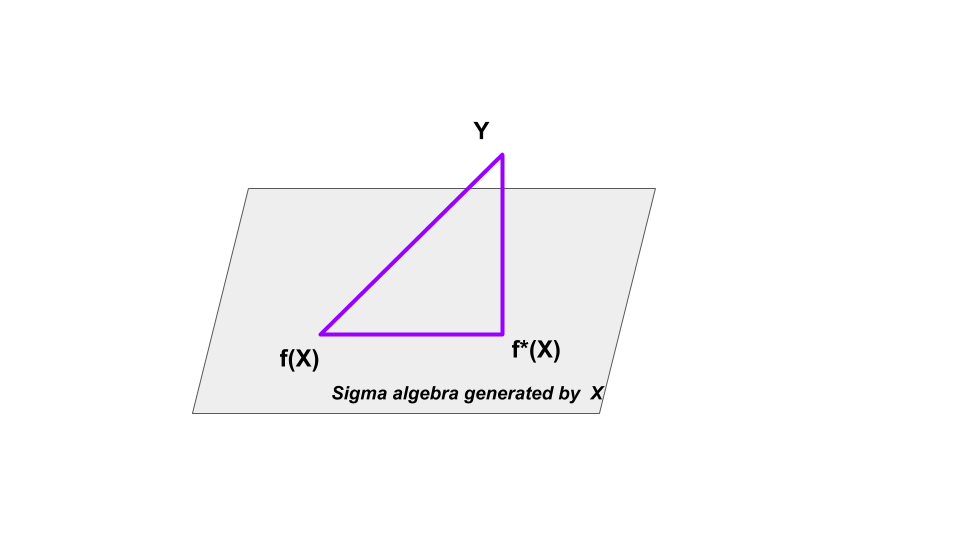
\includegraphics[width=0.8\textwidth]{optimalL2cond.png}
\end{center}


\noindent\rule{\textwidth}{.5pt}

reference for elementary math:
\href{http://www.ee.nthu.edu.tw/cschang/Talk01142008.pdf}
{Understanding Conditional Expectation via Vector
Projection}
}

\frame{

The following exercise is to directly minimize functions in the  function space.

\begin{ex}
Use the method of perturbation  to solve 
\footnote{Rigorously, $f$ is in the $p$-weighted $L_2$
space}

\[
\inf_{f} \iint (f(x)-y)^2 p_{X,Y}(x,y) dx dy
\]
where $p_{X,Y}$ is the joint pdf of the r.v.s $(X, Y)$.
The optimal $f^*$ satisfies 
$$ \int (f^*(x)-y)p_{X,Y}(x,y)dy=0,~~
\quad \forall x$$
i.e., $\e Y = \e f^*(X)$
\end{ex}
What if generalized  the $L_2$ norm to $L_p$ norm ?
\bigskip
}

\frame{
\begin{ex}[Conditional distribution of multivariate Gaussian r.v.]

Suppose that $X=(X_1, X_2)$ is a two dimensional Gaussian random variable with mean $\mu=(\mu_1, \mu_2) $ and the covariance matrix $\Sigma=\left(
  \begin{array}{cc}
    \sigma_1^2 & \rho\sigma_1\sigma_2  \\
    \rho\sigma_1\sigma_2 & \sigma_2^2 \\
  \end{array}
\right) $. What is the conditional pdf $p(x_1|x_2)$ of $X_1$ given $X_2=x_2$? 
What is the expectation of $X_1$ given $X_2=x_2$?
What is the 
\href{https://en.wikipedia.org/wiki/Multivariate_normal_distribution\#Conditional_distributions}{general result} in $n$ dimension ?
\end{ex}

\[
X_1|_{X_2=x_2}\sim \mathcal{N}(\mu_1+\rho\frac{\sigma_1}{\sigma_2}(x_2-\mu_2), \sigma_1^2(1-\rho^2))
\]

}
\frame{
\biz
\item The objective function $\mathcal{E}(f)$ is also called 
loss function, risk, etc.
 \item $\e f^*(X) =\e Y$:  $f^*(X)$ is an unbiased estimate of $Y$;
\item
The variance of the difference between $Y$ and the optimal prediction $f^*(X)$
is
$$\sigma^2_*(x):= \e  \left[(Y-f^*(X))^2 \vert X=x\right]$$ 
  \item
  Take average of $\sigma^2(x)$ over $x$, then
the averaged uncertainty is 
 \[ \sigma^2_* := \e_X  \sigma^2_*(X)=\e  \left[\abs{Y-f^*(X)}^2 \right]=\mathcal{E}(f^*)
 \]
This is the   variance  of the measurement error $Y-f^*(X)$:
\hb{irreducible error}
\eiz
}

\frame 
{{Notations}
We have shown in \eqref{proj-cond-exp-3}
for any two r.v.s  $X, Y$ and an arbitrary function $f$: 
\begin{equation}
 \begin{split}
\Ecal(f)= \underbrace{
\e_{X,Y}(  |f(X)-Y|^2    )}
_{\text{\bf Mean Square Error }}
 & = 
 \underbrace{\e_{X,Y} (  |f^*(X)-Y|^2   )}
 _{=\Ecal(f^*), {\text{\bf Bayes error} } } + 
 \underbrace{
 \e_X\left[ \abs{f(X)-f^*(X)} ^2 \right]
 }
 _{\text{\bf model error} } 
\end{split}
\end{equation}
where $f^*(x)=\e(Y \vert X=x)$ is called {\bf Bayes rule}.\biz
\item Bayes error:  irreducible error;
\item Model error:  the distance from $f$ to 
the optimal prediction $f^*$.
\eiz
\bigskip

Next, \hb{  the same idea,  $\inf_f \Ecal(f)$,  applied to classification problem...}
}

\frame {
\frametitle{ Baye classifier for classification:
optimal for the 0-1 loss}

\begin{itemize}[<+->]
\item Assume $Y \in \{1,\ldots,K\}$ and $X \in {\Real}^p$.
So a function $f:\Xcal \to \Ycal$ is a piece-wise constant function.
\item A loss function $\ell(Y, f(Y))$ for penalizing errors in misclassification.
\item Most Common choice for classification problem is the {\bf  0-1 loss}
\footnote{corresponding to the Dirac delta function }
$$
\ell (Y , f(X))=I(Y \neq f(X))
:=\begin{cases}
1 & \mbox{ if } Y \neq f(X)
\\
0 &   \mbox{ if }   Y = f(X)
\end{cases}.
$$
\item The expected prediction error, or the generalization error, is
$$
\Ecal (f)=\e I(Y \neq f(X))=\p (Y \neq f(X))=1-\p(Y=f(X)).
$$
\item The Bayes rule minimizing $\Ecal(f)$ is
the one maximizing $\p(Y=f(X))=
\int_\Xcal  \p(Y=f(x) \vert X=x) p_{X}(x)\dx$,
which is 
$$
\otherbox{
f^*(x)=\argmax_k \p(Y=k|X=x).
}
$$
since  $\p(Y=k|X=x) \leq \p(Y=f^*(x) \vert X=x ), \forall k $
\end{itemize}

}

\frame{
{Notation for classification}

\biz
\item {\bf Bayes classifier}: the maximizer of 
conditional probability 
\[
f^*(x)=\argmax_k \p(Y=k|X=x).
\]
\item {\bf Bayes error rate}:
the minimal value of $\Ecal$
\[ \inf_{f}\Ecal(f) = \Ecal(f^*)=1- \p(Y=f^*(X))=
1-\int_\Xcal \p(Y=f^*(x))p_X(x)\dx\]
\item  {\bf Bayes decision boundary}

The boundary separating the $K$ partition domains in $\Xcal$
on each of which $f^*(x)$ is constant.
For the binary classification 
($K=2, \Ycal=\set{-1,1}$), 
the boundary  corresponds to
the level set  where $ \p(Y=1\vert X=x)= \p(Y=-1\vert X=x)=0.5$.
\eiz

\bigskip 
\footnotesize{We focus on the regression fit first
and will come back to classification later.
}
}

%%%%--------------------------------
\begin{frame}
\begin{ex}[Ex. 2.2 in ESL]
Let $\Xcal=\Real^2$ and $\Ycal=\set{0,1}$
and the conditional distribution $X \vert Y$ is the normal   
$\mathcal{N}(\mu_Y, (1+Y)I_2)$ where 
$\mu_y= (y,y)^\tr$ for $y\in \Ycal$,
$I_2$ is identify matrix.
Find the Bayes decision boundary
and the Bayes error rate for this problem.
\end{ex}
 

\end{frame}

%%%%--------------------------------


\frame{
{How do we estimate $f^*$ ? }
\biz
\item direction method by definition of conditional expectation
\footnote{or conditional probability for the Bayes classifier}; 
\item optimization method by minimization of generalization error;
\eiz

}
\frame {

\frametitle{Nearest neighbors method to approximate  condition expectation}

A natural way to approximate the function $\e (Y \vert X=x)$ is to 
replace the expectation by the average
from the data $\Dcal=\set{(x_i,y_i)}$:
$$f^*(x)=\e (Y\vert X=x) \approx \mbox{AVE}\set{y_i :  \mbox{ where } ~x_i=x},
~~\forall x\in \Xcal$$
or
$$f^*(x)=\int_\Ycal y\, p_{Y|X}(y;x ) dy $$ 
where $p_{Y|X}(y;x )
=\frac{p_{X,Y} (x,y)}{p_X(x)}$
by estimating the density $p_{X,Y}(x,y)$ first?

Question: Would these work well in practice ? 
 
\pause

(1) this formula is defined point-wisely;
(2) one does not have an accurate estimation of the expectation or the joint distribution $p(x,y)$,
particularly in high dimension.
}
%%% ------
\frame{
{$k$-NN}

\biz 
\item Use windows with size $\Delta$
\[
\e (Y\vert X=x) \approx \mbox{AVE}\set{y_i :  \mbox{ where } ~
\abs{x_i-x} \leq \Delta}
\]

\item Use $k$ -nearest neighbors
(KNN):
have a look at its neighbors,
and take a vote:
$$
\e (Y\vert X=x) \approx \mbox{AVE} \set{y_i :  x_i   \in {\cal N}_k(x) }
$$
where ${\cal N}_k(x)$ is a neighborhood of $x$ that contains exactly $k$ neighbors
(k-nearest neighbors). The number samples in $\mbox{AVE}$
is fixed ($k$).
\eiz 

Two approximations are happening here:
\ben
\item  expectation is approximated by averaging over sample data;
\item conditioning at a point is relaxed to conditioning on some region
``close'' to the target point.
\een

\bigskip
Note: \hb{ A metric on $\Xcal$ is  necessary     here. 
The choice of metric, $|x-x_i|$, is a practical issue.}
}

%%%%--------------------------------------
\frame {

\frametitle{Curse of dimensionality}

k-NN can fail in high dimensions, because it becomes difficult to gather $k$ observations close to a target point $x_0$.
\pause
\begin{itemize}[<+->]
\item Neighborhoods tend to be spatially large, and estimates are
biased.
\item Reducing the spatial size of the neighborhood means reducing $k$, and
the variance of the estimate increases.
\end{itemize}

\pause
In general (see Figure 2.6. [ESL]), when the dimension of $\Xcal$
is very large (the sample size $N$ is fixed.)
\begin{itemize}[<+->]
\item Most points are at the boundary, and points tend to be equidistant (Hall et al., JRSS-B, 2005).
\item Sampling density is proportional to $n^{1/p}$: the number of sample size increases exponentially in dimension $p$: If 100 points are sufficient
to estimate a function in ${\Real}^1$, $100^{10}$ are needed to achieve similar
accuracy in ${\Real}^{10}$.
\end{itemize}
This is similar to the curse of dimensionality in using the mesh grid based method to solve
high dimensional PDE.

}





\frame{

{\color{blue} \huge 

Minimizing the generalization error: learning as minimization}

}
\frame{
\biz
\item Loss function $\ell(y, \hat{y}):  \Ycal  \times \Ycal \to \Real^+\cup\set{0}$
\biz
\item  $L_2$, $L_1$ norm
\item  0-1 loss:  $\ell(y,\hat{y})= I( y\neq \hat{y})$.
\item  ...
\eiz
\item Population risk/loss (Generalization error): $\Ecal (f) = \e \ell (Y, f(X))$
\eiz



\par
The direct  approach  of minimizing the risk \[ \min_{f} \mathcal{E}(f)=
 \e \ell (Y, f(X))\]
where $f$ can be in a very general class of functions, such as
continuous function on $\Xcal$, or even piecewise continuous function.

It is important to specify a  hypothesis space $\mathcal{H}$ to restrict the search space.

\ben

\item 
the function space of $f$  to search:  \hb{ hypothesis space(model class)} $\mathcal{H}$.



\item approximate the expectation $\e$ in $\mathcal{E}$ with  the use of data $\Dcal=\set{x_i, y_i}$.
\een


}
\frame{
%{hypothesis space and training error}
{Notations}
\ben

\item 
 
 The minimizer  of $$\min_{f\in \mathcal{H}}\mathcal{E}(f)$$
is denoted by $f_{\mathcal{H}}$. 
 

\item  
Population loss/risk is approximated by 
{\bf empirical} loss/risk associated with $\Dcal=\set{(x_i, y_i): i=1,\ldots,N}$:
\[
\mathcal{E}(f) = \e \left [ \abs{Y-f(X)}^2\right]
\approx 
\mathcal{E}_N(f)=\frac{1}{N} \sum_ i \ell (y_i, f(x_i))  
\]
The learning algorithm produces the  learnt function  $ \hat{f}_\Dcal $
(\hb{ regression function})
as the  solution to  $$
\Ecal_N ( \hat{f}_\Dcal ) = \min_{f\in \Hcal}\mathcal{E}_N(f)=
\min_{f\in \Hcal} \frac{1}{N} \sum_{(x_i,y_i)\in \Dcal}\ell(y_i,f(x_i))$$
\biz
\item 
The {\bf training error} is   $\mathcal{E}_N(\hat{f}_\Dcal)$ .
\item
  The {\bf test error/prediction error} is   $\mathcal{E}(\hat{f}_\Dcal)
  =\e_{X,Y}\ell (Y,\hat{f}_\Dcal(X))$.
  \item The expected test/prediction error is
  $\e_\Dcal  \left[ \mathcal{E}(\hat{f}_\Dcal) \right ]$, which requires
 running on several (statistically identical) datasets  $\sim\Dcal$.
\eiz
\een


}

\frame{


\biz
\item $f_\Hcal$ may not equal to $f^*$ unless 
the ground truth $f^*\in \Hcal$;
\item
$\hat{f}_\Dcal$ depends on {\it three} elements:
 the hypothesis space $\Hcal$,  the (training) data $\Dcal$ ( random ! ) and  the loss function $\ell$.
So, $\hat{f}_\Dcal$ is a random function to approximate the ground truth $f$.
\item
For the fixed $\Hcal$ and $\ell$,  $\hat{f}_\Dcal$ is essentially a mapping from $\Dcal$ to the function space
$\Hcal$.
 As $N\to \infty$, $\hat{f}_\Dcal \to  f_{\Hcal}$ by the law of large number.
\eiz
}
 
\frame{
{Hypothesis space: representation of the function $f$}
\biz
\item parametric approach:  e.g. $f(x)=\theta\cdot x$ with a set of finite and (usually fixed) number of parameters
$\theta$
\item non-parametric approach: functional analysis viewpoint, $f$ is only in some function space.
(such as in the traditional computational math for representing the solution to some PDE )
\item there is no rigorous boundary between parametric/non-parametric: eventually 
the computer represents a function $f$ only by a finite number of freedoms. 
\item need to be restricted to certain model class in practice. Examples:   linear model,  polynomial, spline, kernel machine,   neural network, etc.
\eiz 
}



\frame {

\frametitle{some examples of $\Hcal$}

\begin{itemize}[<+->]
\item Linear function (chapter 3 , ESL)
\item Basis functions and dictionary methods (chapter 5, ESL)
$$
f_{\theta}(x) = \sum_{m=1}^M \theta_m h_m(x),
$$
where $h_m$'s are pre-specified basis functions.
\item Kernel methods and local regression (chapter 6, ESL)
$$
RSS(f, x_0) = \sum_{i=1}^n K(x_0,x_i) (y_i-f(x_i))^2,
$$
where $K$ is a kernel measuring the closeness between points.
\item Roughness penalty (chapter 5, ESL)
$$
\mbox{Penalized RSS}(f; \lambda) = \mbox{RSS}(f) + \lambda J(f),
$$
where $J(f)$ is a regularization term on the model complexity.
\end{itemize}

}

\frame{
\underline{The generalization  error   is  then decomposed into} 
\bigskip
\[
\otherbox
{
\Ecal(f^*) = 
\underbrace{ {\Ecal(f^*) - \Ecal(f_\Hcal) }}_\text{\bf approximation error}
+ \underbrace{{\Ecal(f_\Hcal)- \Ecal_N(\hat{f}_\Dcal)} }_\text{\bf sampling error}
+  
\underbrace{\Ecal_N(\hat{f}_\Dcal)}_\text{\bf training error}
}
\]


}


\frame{

\biz
\item 
Approximation error:
characterized how large (complex)
the hypothesis space $\mathcal{H}$ is.
analogy to the interpolation 
inequality in finite element method.
A larger space of $\Hcal $ indicates
\biz
\item
A  larger effective dimension of this space;
\item A smaller approximation error;
lower bias
\item More difficult for numerical optimization;  
\eiz

\item 
Sampling error:
vanishes if the number of data
points $N$ goes to infinity. This error may be analyzed by
probability inequality 
(e.g. Chebychev);
analysis method used for 
Monte Carlo  simulation.
A larger sample size for training data indicates:
\biz
\item Smaller sampling error; lower variance; 
\item more challenges for data collection and  Big Data techniques;
\eiz
\item  
Training error: 
\biz
\item design of optimization method, numerical convergence rate,
\item  the time and memory cost ... 
\item the output is  a further approximation to $\hat{f}_\Dcal$:
the optimization algorithm stops with a time cost $T$:
$\hat{f}_{\Dcal}^{(T)}$
\eiz 
 \eiz
 }
 
 %%%--------------------------------------
\frame{
{Very Important Remarks }

\biz
\item Although different fields focus on
each of three errors separately,
to address the problems in machine learning 
needs  trans-disciplinary efforts:
\biz
\item approximation theory
\item statistical learning
\item computation  
\eiz
A   joint strategy  is very important to have
a complete picture of the machine learning problem.
 
 
\hb{A small value of training error  $\Ecal_N(\hat{f}_\Dcal)$
does not imply a small value of  $\Ecal(\hat{f}_\Dcal)$. 
}

\item  These three topics are not completely separate.
 For example, the necessary number of sample size $N$
 may depend on the complexity of hypothesis space,
 which further depends  on the  dimension of $\Xcal,\Ycal$
 and the specific representation form of functions in $\Hcal$. 
\eiz
}


\frame{{Generalization Gap}
The optimal function in theory is $f^*$; 
the  optimal function in practical computation is 
$\hat{f}_\Dcal$. The difference in  risks 
of these two:
\[
 \Ecal(\hat{f}_\Dcal) - 
\Ecal(f^*)
\]
is called {\bf generalization gap}:
it measures to which extent 
the performance of the algorithm
learnt from a given training data set $\Dcal$
is valid for the whole distribution $p(x,y)$.

\bigskip
Remark
\biz
\item 
$ \Ecal(\hat{f}_\Dcal) - 
\Ecal(f^*) $ can be either positive or negative;
\item 
$ \Ecal(\hat{f}_\Dcal) - 
\Ecal(f^*) $ still depends on $\Dcal$.
One can use the expected 
$ \e_{\Dcal} \left [
\Ecal(\hat{f}_\Dcal) - 
\Ecal(f^*) 
\right ] $ to represent the average.
\eiz
}
%%%---------
\frame{
{First inequality for Generalization Gap}
\begin{ex}
Prove the upper bound of the generalization gap: 
 \[
 \begin{split}
 \otherbox{
 \abs{ \Ecal(\hat{f}_\Dcal) 
 - \Ecal(f^*)
 }
% =
% \Ecal(\hat{f}_\Dcal) - 
%\Ecal_N(\hat{f}_\Dcal)
%+
%\Ecal_N (\hat{f}_\Dcal)
%-
%\Ecal_N (f^*)
%+\Ecal_N (f^*)
%- \Ecal(f^*)
\leq 2 \sup_{f\in \Hcal} \abs{ \Ecal_N (f)- \Ecal(f)}
}
\\
\approx 2 \sup_{f\in \Hcal}  \frac{1}{\sqrt{N}} 
\sqrt{\var (\ell(Y,f(X)))}
\end{split}
 \]
  \end{ex}
}

\frame{
 
  
 
 
 
~{Limitation of the previous boundedness}:
\biz
\item The first RHS depends on the hypothesis space
 $\Hcal$ and the dataset $\Dcal$ of size $N$ in $\Ecal_N$;
 and the second depends on $\Hcal$ and the joint distribution $p(x,y)$
 of $(X,Y)$.   The ``$\approx$'' is due to the central limit theorem.
 
 \item 
The $\var$ in RHS is w.r.t.  $\Dcal$, and eventually for $p_{X,Y}$.
 \item 
 The supremum in the above inequality
 can describe the {\bf complexity } of  hypothesis space $\Hcal$,
 which increases when $\Hcal$ is ``larger''.
 
 \item
Although this upper bound 
 is quite useful and not  too far way from the true gap;
 but it is not sharp in many cases and fail to serve as 
 a good indicator of the generalization gap.
 A good lower bound is extremely difficult to obtain.
 
  \item $\Ecal(\hat{f}_\Dcal)$ 
  depends on $\Dcal$. When $\Dcal$ is regarded as random,
$\Ecal(\hat{f}_\Dcal)$ is also random.

\eiz
}

\frame{

{\color{blue} \huge 
Statistical  Learning:
Viewpoint of Bias-Variance
Trade-off}
}

\frame{
\bigskip 
\biz
\item
In the approximation theory above,
the introduction of the dataset $\Dcal$ is only used to   
approximate the expectation
w.r.t. the generic r.v.s $X, Y$ 
by their sample average:
population risk $\To$ empirical risk.
\item
In statistical learning, 
$\Dcal$ is regarded as random, 
then $\hat{f}_\Dcal(\cdot)$ is a random function on $\Xcal$,
then  its prediction ability, measured by 
$\Ecal (\hat{f}_\Dcal)$,
is random.
Then it makes sense to consider
\[ \e_{\Dcal} \Ecal (\hat{f}_\Dcal) \]
\eiz
}
\frame{
{Bias-Variance Decomposition / Trade-off}



Let $f$ be a given deterministic function (ground truth)
$\mathcal{X}\to\mathcal{Y}$.

Assume that the response r.v. 
$Y$ is defined by the 
 {additive error 
statistical model}: 
\[
Y=f(X)+\eps
\]
where  the 
r.v.  $\eps$ is independent of $X$
and has mean $0$ and variance $\sigma_\eps^2$.

Assume this model generates on the {training} dataset $\Dcal=\set{(x_i, y_i):1\leq i\leq N}$, i.e.,  $y_i=f(x_i)+\eps_i$ and $\eps_i  \sim \eps$
($\e \eps=0, \var(\eps)=\sigma^2$).
Assume  one learns a  function based on $\Dcal$, 
still denoted by 
$\hat{f}_\Dcal(\cdot)$.
\footnote{it does not have to be
the one in previous part associated with $\Ecal_N$.
For example, $\hat{f}_\Dcal$ can be the $k$-NN model.} 

The key question is 
the prediction performance of this function $\hat{f}_\Dcal$
on a new data $(x_0, y_0)$ where  $x_0\in\Xcal$ is arbitrary and $y_0=f(x_0)+\eps_0$
with the new measurement error $\eps_0$
being independent of 
 $\Dcal$ and distributed as $\eps$.

}

%%%--------
\frame{ {Decomposition of expected prediction 
(squared) error}
The  {\bf expected prediction error} 
(generalization error)
in terms of $L_2$ criterion,
at a new input value $x_0$ is  
\begin{align*}
& \e [  ( Y-\hat{f}_\Dcal(X))^2
\vert X=x_0] 
=
 \e_{\eps_0, \Dcal}   ( f(x_0)+\eps_0-\hat{f}_\Dcal(x_0))^2
 ~~\\
=&\sigma_\eps^2+ \e_\Dcal   \left( f(x_0)-\hat{f}_\Dcal(x_0)\right)^2
~~\because   \e (\eps_0)=0 , \mbox{ and } \Dcal \perp \eps_0
\\
=&
\sigma_\eps^2+ \e_\Dcal   \left( f(x_0)-
\e\hat{f}_\Dcal(x_0) + \e \hat{f}_\Dcal(x_0)- \hat{f}_\Dcal(x_0) \right)^2 \\
=&
\otherbox{
\sigma_\eps^2+ 
\underbrace{ ( f(x_0)-
\e_\Dcal \hat{f}_\Dcal(x_0))^2}
_\text {Bias$^2$}
 + 
 \underbrace{
 \var_{\Dcal} (\hat{f}_\Dcal(x_0))
 } _\text{Variance}}
\end{align*}
Here the subscripts emphasize the random elements to take expectation.
$\sigma^2_\eps=\var(\eps_0)$ is the \hb{irreducible} uncertainty of the new measurement error.
\begin{den}
 $\hat{f}_\Dcal$ is called {\bf unbiased}
if the functions $\e_{\Dcal} \hat{f}_\Dcal (x)$ and $f(x)$ are equal.
\end{den}
}

%%%------------------------------------------
\frame{ 

Sometimes, this quantity is further  taken expectation for 
 $x_0$ w.r.t.  $p_X$.

 Use the generic r.v. $(X,Y=f(X)+\eps)$ for a new {\bf testing} pair,
 which is independent of the training set $\Dcal$:

 \begin{align*}
&\e_{X,Y}  \left[ \e_{\Dcal}  \left(Y- \hat{f}_\Dcal(X)\right)^2 \right]\\
=&\e_{X,\eps, \Dcal} 
\left(f(X)-\hat{f}_\Dcal(X) + \eps
\right)^2
\\
=&\sigma_\eps^2+ \e_X
 \left(
 f(X) - \e_\Dcal \hat{f}_\Dcal(X)
 \right)^2
 +\e_X \left[ \var_{\Dcal} (\hat{f}_\Dcal(X)  
 \right].
\end{align*}
This is simply equal to  $ \e_\Dcal \Ecal (\hat{f}_\Dcal) = 
\e_{\Dcal} \e_{X,Y} \abs{Y-\hat{f}_\Dcal(X)}^2 $.
 
 \bigskip
  The variance term 
 $ \var_{\Dcal} (\hat{f}_\Dcal(x_0))
$ is typically $\sim \frac{1}{N}\times C$ for which 
$C$ may depend on complexity of the model space $\Hcal$.


  }
 


%%%------------------------------------------
 
\frame{
%For linear regression:
%\[ \Var (\hat{f}_\Dcal(x_0))
%\sim p\sigma^2_\eps/N  \]
%where $p$ is the number of components,
%i.e.,  the dimension 
%of $X$. $\mathcal{X}=\Real^p$.
%

\biz
\item 
low bias:  large model space, 
low training error, 
overfitting, bad generalization ability
(high variance);
 \item low variance:  
rigid model space,
insensitive to the perturbation of the dataset used in fitting;
good generalization for the new data from the same distribution. 
\item BAD news:
it is almost impossible to decrease the bias and variance terms
simultaneously!

 \item Criteria for model assessment or variable selection:
{
\color{blue}\bf good trade-off between the bias and variance
}

\biz
\item Analyse the bias or variance 
or model complexity to have analytical 
results (very limited cases)
\item  
A practical method is to estimate $\e [  ( Y-\hat{f}_\Dcal(X))^2]
\approx \frac{1}{n} \sum_j (Y'_j-\hat{f}_\Dcal(X'_j))^2$
where $X'_j$ are not from $\Dcal$
but an independent dataset $\Dcal'$.
\item Where is the ``new'' dataset $\Dcal'$?
cross-validation
(split 1 cent into 1/2 cents)  and bootstrap
(1 cent used twice ) .

\eiz


\eiz
}

%%%------------------------------------------------------
\frame{
\begin{center}
\begin{figure}
\includegraphics[width=.8\textwidth]{bias-variance-tradeoff.png}
\caption{  Bias-Variance Tradeoff as a Function of Model Capacity/Complexity
}
\end{figure}
\end{center}
}


%%%------------------------------------------------------
\frame{
\begin{center}
\begin{figure}
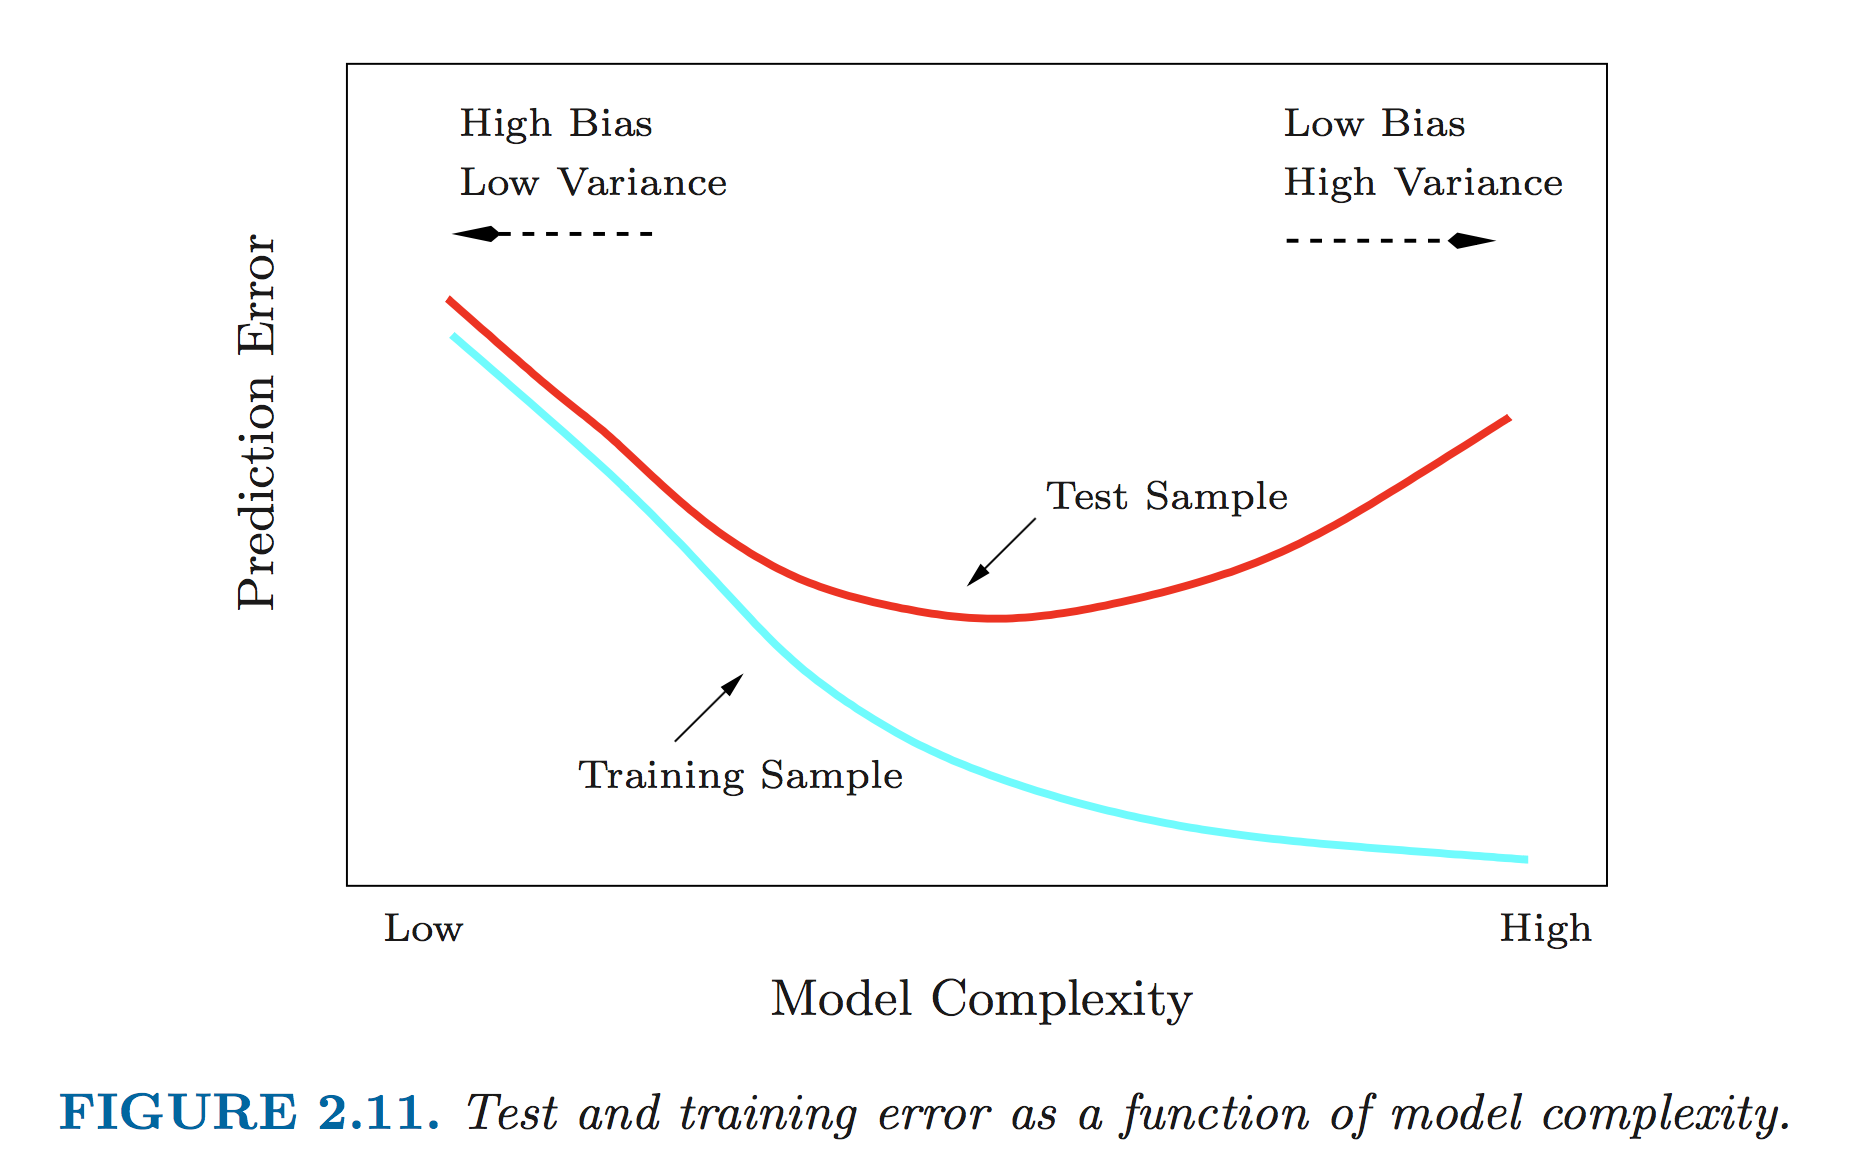
\includegraphics[width=.98\textwidth]{Fig2_11.png}
\end{figure}
\end{center}
Exercise:  Prove that  the blue curve is always below 
the red curve. (Ex. 2.9 in [ESL])
}


%%%------------------------------------------------------

\frame{ {Application of Bias-Variance decomposition
to $k$-NN}

Consider the $k$-nearest-neighbor regression fit 
to the data $\Dcal=\set{(x_i,y_i)}$
arising from the additive model $Y=f(X)+\eps$: 
$$\hat{f}_\Dcal^k(x)=\frac{1}{k}\underset{x_i \in N_k(x)}\sum   y_i
=\frac{1}{k}\underset{x_i \in N_k(x)}\sum   (f(x_i) +\eps_i) .$$
WLOG, we assume that the input design points $\set{x_i}$ in
the training $\Dcal$ is 
deterministic. Then the expectation w.r.t. $\Dcal$
is only for the measurement errors $\eps_i$:
\biz
\item 
The bias is $f(x_0)-\e_\Dcal [\hat{f}^k_\Dcal  (x_0)]=
f(x_0)-
\frac{1}{k}  \underset{x_i \in N_k(x_0)}\sum   f(x_i)$;
\item 
The variance is $\var_{\Dcal} ( \hat{f}^k_\Dcal  (x_0) )
=\frac{1}{k}\sigma^2_\eps$
\eiz
\begin{ex}
Assume $x_0=0$, $x_i=i/N, ~~i=1,2,\ldots N$.
Compute the $\mbox{EPE}(k)$, the expected prediction error, 
as a function of  $k$ and fine the optimal $k^*$ 
in this special case.
\end{ex}

}


%%%------------------------------------------------------


\frame {

\frametitle{Model Assessment: practical techniques}

Typical objectives:
\ben
\item Choose a value of a tuning parameter  (\hb{hyperparameter})
used in the model
(such as $k$ in k-NN)
\item Estimate the prediction performance  (test error) of a given model
\een
\vspace{3mm}
Remarks:
\begin{itemize}
\item For both objectives, the best approach is to run the procedure on
an independent test set, if one is available.
\item If possible, one should use different test data for (1) and (2) above: a
{\it validation set} for objective (1) and a {\it test set} for  objective (2).
\item Often there is insufficient data to create a separate validation or test set. In this case, {\it Cross-Validation} is useful.
\end{itemize}

}



%%%--------------------------------------------------------------------

\frame {

\frametitle{K-fold cross validation}
Denote the hyper-parameter by $\lambda$.
K-fold cross validation is the most popular method for estimating a tuning parameter $\lambda$. 

\vspace{3mm}
Divide the dataset (of size $N$) into $K$ subsets: ${\cal A}_1,\ldots,{\cal A}_K$ ($K=2,5,10$ or $N$)
\begin{itemize}
\item For each $k = 1, \ldots, K$, fit the model with parameter $\lambda$ to $\{{\cal A}_1,\ldots,{\cal A}_{k-1},{\cal A}_{k+1},\ldots,{\cal A}_K\}$ giving $ {f}^{-k}_\lambda(\cdot)$, and compute its prediction error on ${\cal A}_k$: $$E_k(\lambda)=\sum_{x_i \in {\cal A}_k} \ell (y_i, f^{-k}_\lambda(x_i)).$$
\item The average of these $K$ values $E_k(\lambda)$ give  the cross-validation error (per sample)
    $$
    CV(\lambda):=\frac{1}{N} \sum_{k=1}^K E_k(\lambda).
    $$
\item Choose the optimal $\lambda^*$ yielding the smallest $CV(\lambda)$.
\end{itemize}

}



%%%--------------------------------------------------------------------

\frame {

\frametitle{K-fold cross validation}

\begin{itemize}
\item Cross-validation is often abbreviated as CV.
\item In the subset selection procedure, $\lambda$ is the subset size
\item $f^{-k}(\lambda)$ is the  best model of size $\lambda$, found from the training set that leaves out the $k$-th part of the data
\item $E_k(\lambda)$ is its estimated test error on the $k$-th part.
\item Using $K$-fold CV, the $K$ test error estimates are averaged to give the final CV estimated test error.
\item The output is the model associated with  $\lambda^*$,
typically, 
computed  by using all $N$ data. 
\end{itemize}

}



%%%--------------------------------------------------------------------

\frame {

\frametitle{Bootstrap}

\begin{itemize}
\item Bootstrap works by sampling $N$ times with replacement from the training set to form a ``bootstrap" data set. Then model is estimated on the bootstrap data set,
and predictions are made on the original training set.
\item This process is repeated many times and the results are averaged.
\item {\it Bootstrap is most useful for estimating standard errors of predictions.}
\item Can also use modified versions of the bootstrap to estimate prediction error. Sometimes produces better estimates than CV (still an open question!)
\end{itemize}

}



\end{document}


